% 2.25, 2.26, 2.38

% List notation theorems
% addend-subset theorem
% pf uniquness
% pf of product
% Division-subset theorem (2.12)
% Cardinality of equal lists
% Cardinality of sum
% GCD-intersection theorem
% LCM-union theorem
% Identity property
% coprime-disjoint theorem
% pf of fraction
% min(a, b) = a \vee min(a, b) = b

\item Theorem: $n \in \mathbb{N} \wedge n \neq 1 \rightarrow \exists p (p \in \mathbb{P} \wedge p \mid n)$

But first, Prime or composite lemma: Any natural number $p$ greater than one is either prime or composite. In other words if $p$ is not composite, it is prime. If $p$ is not prime, it is composite.

\textit{Every now and then, I feel I need to prove one thing formally so I don't get to relaxed with my form.}

\begin{proof}
$p$ is not composite & Premise \\
$\neg \exists a, b \in \mathbb{N} (p = ab \wedge 1 < a, b < p) $ & Definition of composite (negated) \\
$\neg \exists a, b \in \mathbb{N} (p = ab \wedge 1 < a < p) $ & Simplification \\
$\forall a, b \in \mathbb{N} \neg(p = ab \wedge 1 < a < p) $ & Quantifier exchange \\
$\neg (p = ab \wedge 1 < a < p) $ & Universal instantiation \\
$\neg (p = ab) \wedge \neg (1 < a < p) $ & DeMorgan's law \\
$p = ab \rightarrow \neg (1 < a < p) $ & Conditional disjunction \\
$p = ab \rightarrow \neg (1 < a \wedge a < p) $ & Property of inequality \\
$p = ab \rightarrow \neg (1 < a) \vee \neg (a < p) $ & DeMorgan's law \\
$p = ab \rightarrow 1 \geq a \vee a \geq p $ & Property of inequality \\
$p = ab \rightarrow (1 = a \wedge a \geq p) $ & Property of Natural numbers \\
$p = ab \rightarrow (1 = a \wedge a = p) $ & $a \mid p \rightarrow a \leq p$ \\
$a \mid p \rightarrow (1 = a \wedge a = p) $ & Definition of division \\
$\forall a (a \mid p \rightarrow (1 = a \vee a = p))$ & Universal generalization \\
$p$ is prime & Definition of primes
\end{proof}

\begin{proof}
$p \in \mathbb{P}$ & Premise \\
$\neg (\forall d (d \mid n \rightarrow (d = 1 \vee d = n)))$ & Definition of prime \\
$\exists d \neg (d \mid n \rightarrow (d = 1 \vee d = n))$ & Quantifier exchange \\
$\exists d \neg (\neg(d \mid n) \vee (d = 1 \vee d = n))$ & Conditional disjunction \\
$\exists d \neg \neg (d \mid n) \wedge \neg (d = 1 \vee d = n)$ & DeMorgan's law \\
$\exists d (d \mid n \wedge \neg (d = 1 \vee d = n))$ & Double Negation \\
$\exists d (d \mid n \wedge d \neq 1 \wedge d \neq n)$ & DeMorgan's law \\
$\exists d (d \mid n \wedge 1 < d < n)$ & Inequality over naturals \\
$\exists d \exists c (cd = n) \wedge 1 < d < n$ & Definition of divides \\
$\exists d \exists c (cd = n \wedge 1 < c < n) \wedge 1 < d < n$ & Inequality over naturals \\
$p$ is composite
\end{proof}

Because of this, let $a \notin \mathbb{P}$ stand for `$a$ is composite' (only when $a \neq 1$).

Transitivity of divisibility Lemma: $a \mid b \wedge b \mid c \rightarrow a \mid c$

\begin{proof}
$an = b$ & Definition of divides \\
$bm = c$ & Definition of divides \\
$anm = c$ & Substitution \\
$a \mid c$ & Definition of divides
\end{proof}

Theorem: $n \in \mathbb{N} \wedge n \neq 1 \rightarrow \exists p (p \in \mathbb{P} \wedge p \mid n)$

\begin{proof}
Assume: $p \in \mathbb{P}$ & \\
$p = 1p$ & Identity of Multiplication \\
Conclude: $p \mid p$ & Definition of divides $\square$ \\
Otherwise: $p \notin \mathbb{P}$ \\
Follow this algorithm: \\
\textbf{Initial step:} \\
$p = a_1 b_1 \wedge 1 < a_1, b_1 < p \fs a_1, b_1$ & Definition of composite ($\notin \mathbb{P}$) \\
$a_1 \mid p$ & Definition of divides \\
If $a_1 \in \mathbb{P}$: halt \\
Otherwise: $a_1 \notin \mathbb{P}$ \\
$a_1 = a_2 b_2 \wedge 1 < a_2 < a_1 < p$ & Definition of composite \\
Repeat with \(a_1 \gets a_2\) \\
\textbf{\(i\)th step} \\
$a_i = a_{i+1} b_{i+2} \wedge 1 < a_i < a_{i-1} < \underbrace{\dots}_{i \mathrm{~times}} < p$ & Definition of composite \\
$a_{i+1} \mid a_{i}$ & Definition of divides \\
If $a_i \in \mathbb{P}$ halt \\
Otherwise $a_i \notin \mathbb{P}$ and repeat\\
\textbf{Result:} \\
$a_{n - 1} = a_n b_n \wedge 1 < a_n < \underbrace{\dots}_{p \mathrm{~times}} < p$ \\
There can not be $p$ unique numbers between $1$ and $p$\\
Therefore this process must terminate (call that place $a_j$) & Algorithm halts\\
$a_j \in \mathbb{P} \wedge a_j \mid a_{j-1} \wedge a_{j-1} \mid a_{j-2} \wedge \dots \wedge a_1 \mid p$ & Condition for termination \\
$a_j \in \mathbb{P} \wedge a_j \mid p$ & Transitivity of divisibility lemma
\end{proof}

\item $\{2, 3, 5, 7, 11, 13, 17, 19, 23, 29, 31, 37, 41, 43, 47, 51, 53, 59, 61, 67, 71, 73, 79, 83, 89, 97\}$

\item Theorem: $n \in \mathbb{P} \leftrightarrow \neg \exists p (p \in \mathbb{P} \wedge 1 < p \leq \sqrt{n} \wedge p \mid n)$

I will simply prove the biconditional with both sides negated.

Theorem equivalent: $n \notin \mathbb{P} \leftrightarrow \exists p (p \in \mathbb{P} \wedge 1 < p \leq \sqrt{n} \wedge p \mid n)$

\begin{proof}
$\rightarrow$ \\
$n \notin \mathbb{P}$ & Premise \\
$ab = n \fs 1 < a, b < n$ & Definition of $\notin \mathbb{P}$ \\
Assume the following for contradiction \\
$a > \sqrt{n}$ & Assume \\
$b > \sqrt{n}$ & Assume\\
$n > 1$ & Premise \\
$\sqrt{n} > 1$ & Property of square root \\
$a > \sqrt{n} > 1$ & \\
$b > \sqrt{n} > 1$ & Property of inequality\\
$ab > n$ & Property of inequality \\ & (since they are all greater than 1) \\
$ab = n$ & Definition of $a$ and $b$ \\
$\neg (a > \sqrt{n}) \vee \neg (b > \sqrt{n})$ & Contradiction \\
$a \leq \sqrt{n} \vee b \leq \sqrt{n}$ & Property of inequality \\
Either way: \\
$\exists p (1 < p \leq \sqrt{n} \in \mathbb{N})$ & Existential instantiation\\ &(on $a$ or on $b$)
\end{proof}

\begin{proof}
$\leftarrow$ \\
$p \in \mathbb{P} \wedge 1 < p \leq \sqrt{n} \wedge p \mid n$ & Universal instantiation \\
$\sqrt{n} < n$ & Property of positive numbers \\
$1 < p < n$ & Property of inequalities \\
$\exists c (1 < c < n \wedge pc = n)$ & Definition of divides \\
$1 < p, c < n \wedge pc = n$ & Restatement \\
$n \notin \mathbb{P}$ & Definition of composite
\end{proof}

\item 
$101 < 121$ \\
$\sqrt{101} < \sqrt{121}$ since they are all positive \\
$\sqrt{101} < 11$ \\
$\{p \mid p \in \mathbb{P} \wedge p < 11\} = \{2, 3, 5, 7\}$ \\
$2 \nmid 101 \wedge 3 \nmid 101 \wedge 5 \nmid 101 \wedge 7 \nmid 101$ \\
$\therefore 101 \in \mathbb{P}$

\item 
\newcommand*\circled[1]{
\tikz[baseline=(char.base)]{
\node[shape=circle,draw,inner sep=1pt] (char) {#1};
}
}

\begin{python}[tools.py]
output = r'$\{$'
for x in range(2, 101):
    if is_prime(x):
        output += r'$\circled{{{x}}}$, '.format(**locals())
    else:
        output += r'$\cancel{{{x}}}$, '.format(**locals())
output = output[:-2]
output += r'$\}$'
print output
\end{python}

\item 
The blue line is $\frac{\Pi(x)}{x}$.

The green line is $\frac{1}{\ln(x)}$

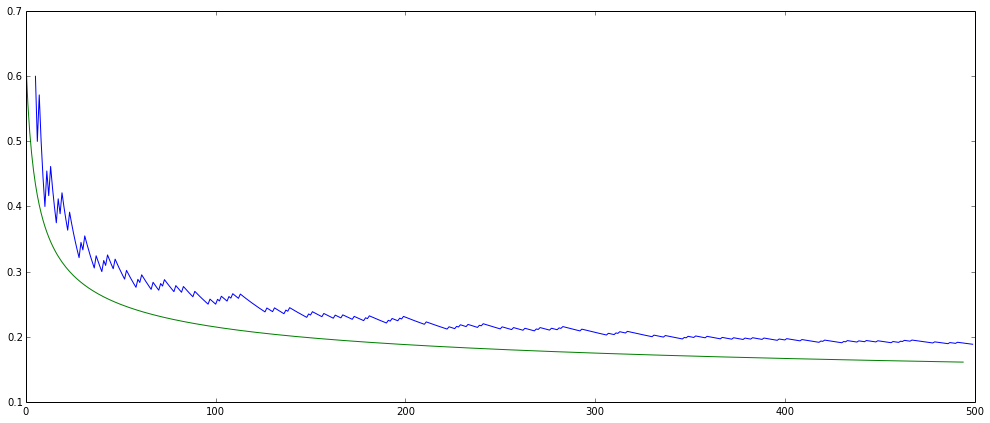
\includegraphics[width=6in]{primes_small.png}

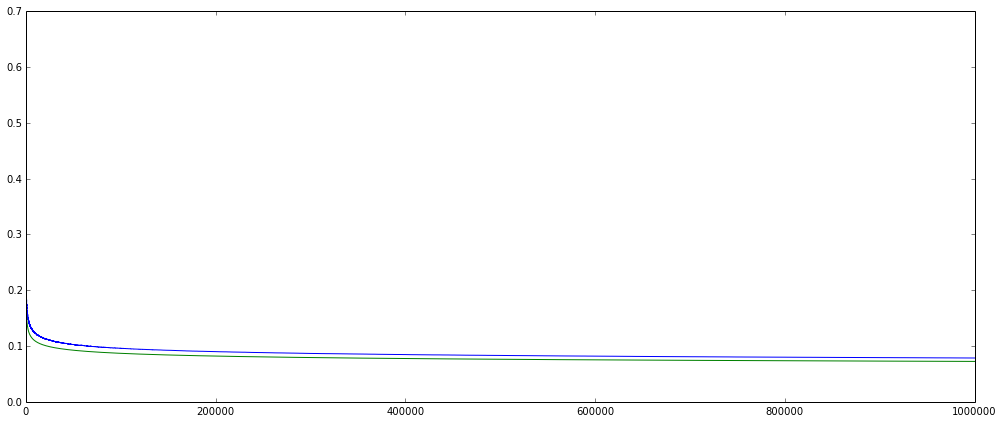
\includegraphics[width=6in]{primes_large.png}

\item Theorem: Every natural number \(n\) excluding one can be written as the product of primes \(\{p_1, p_2, \dots, p_m\}\) (not necessarily all unique). (In other words \(n = p_1 p_2 \dots p_m\).)

\begin{proof}
\(n \in \mathbb{N} \wedge n \neq 1\) & Premise \\
\(\exists p_1 (p_1 \mid n)\) & Theorem 2.1 \\
\(\frac{n}{p_1} = 1 \vee \frac{n}{p_1} \neq 1\) & Excluded Middle \\
&\(\frac{n}{p_1}\) is legal since \(p_1 | n\) \\
Assume: \(\frac{n}{p_1} = 1\) \\
Conclude: \(n = p_1\) & Algebra \\
Otherwise: \(\frac{n}{p_1} \neq 1\) \\
Conclude: \(\exists p_2 (p_2 \mid \frac{n}{p_1})\) & Theorem 2.1 \\
Follow this algorithm: \\
\textbf{Initial step:} \\
If \(\frac{n}{p_1 p_2} = 1\): \\
Conclude: \(p_1 p_2 = n\) \\
Otherwise: \(\exists p_3 (p_3 \mid \frac{n}{p_1 p_2})\) & Theorem 2.1
Repeat with \(\frac{n}{p_1 p_2} \gets \frac{n}{p_1 p_2 p_3}\) \\
\textbf{\(i\)th step:} \\
If \(\frac{n}{p_1 p_2 \dots p_i} = 1\): \\
Conclude: \(p_1 p_2 \dots p_i = n\) \\
Otherwise: \(\frac{n}{p_1 p_2 \dots p_i} \neq 1\) \\
\(\exists p_{i + 1} (p_{i+1} \mid \frac{n}{p_1p_2})\) & Theorem 2.1\\
\textbf{Result:} \\
Each iteration, \(n\) decreases.\\
Therefore the algorithm halts. \\
\(p_1 p_2 \dots p_m = n\) & Halting condition
\end{proof}

Note that I don't have exponents on the primes because I am letting them be necessarily unique. It is easier to prove this way.

\item Theorem: \(p k = q_1 q_2 q_3 \dots q_mn \wedge p \in \mathbb{P} \wedge \forall i (q_i \in \mathbb{P}) \rightarrow \exists i (p = q_i)\)

Coprime primes lemma: any prime number ($p$) is coprime to any other prime number ($q$).

\begin{proof}
\(p \in \mathbb{P} \wedge q \in \mathbb{P} \wedge p \neq q\) & Premise \\
$\gcd(p, q) \mid p \wedge \gcd(p, q) \mid q $ & Definition of GCD \\
$(a = 1 \vee a = q) \wedge (a = 1 \vee a = p)$ & Definition of prime \\
$a = 1 \vee a = p = q$ & Simplification \\
$p \neq q$ & Premise \\
$a = 1$ & Disjunctive syllogism
\end{proof}

\begin{proof}
$p \neq 1$ & Premise \\
$p \mid (\prod\limits_{i=1}^{n} q_i)$ & Definition of divides \\
$\forall i \{ q_i \neq p\}$ & Assume for contradiction \\
$\forall i \{ (q_i, p) = 1\}$ & Coprime primes lemma (applied over all $p_i$) \\
$p \mid q_1 \prod\limits_{i = 2}^n q_i$ & Algebra \\
$(p, q_1) = 1$ & Coprime primes lemma \\
$p \mid \prod\limits_{i=2}^n q_i$ & Theorem 1.41 (Base case) \\
$p \mid \prod\limits_{i=j}^n q_i$ & Assume (Inductive hypothesis) \\
$p \mid q_{j+1} \prod\limits_{i=j+1}^n q_j$ & Algebra \\
$(p, q_j) = 1$ & Coprime primes lemma \\
$p \mid \prod\limits_{i=j+1}^n$ & Theorem 1.41 (Inductive Step)\\
$p \mid \prod\limits_{i=n}^n$ & Inductive axiom \\
$p \mid 1 \wedge p \neg \mid 1$ & Product rule \\
$\neg \forall i \{ q_i \neq p\}$ Contradiction \\
$\exists i\{ q_i = p\}$ & Quantifier Exchange
\end{proof}

\item Theorem: Every natural number excluding one has a \textbf{unique} prime factorization. Given a natural-number \(n\) greater than one, if \(n = p_1 p_2 \dots p_m = q_1 q_2 \dots q_s\) then \(\forall p_i \exists q_j (p_i = q_j) \wedge \forall q_j \exists p_i (p_i = q_j)\).

\begin{proof}
\(p_1 p_2 p_3 p_4 \dots p_m = q_1 q_2 q_3 q_4 \dots q_s\) & Premise \\
\(\exists i (p_1 = q_i) \wedge p_2 p_3 p_4 \dots p_m = q_1 q_2 q_3 q_4 \dots q_{i - 1} q_{i + 1} \dots q_s\) & Lemma 2.8 \\
\(p_1 = q_1 \wedge p_2 p_3 p_4 \dots p_m = q_2 q_3 q_4 \dots q_s\) & Reordering \\
& I am allowed to write the list in any order \\
& So I choose to write the matching \(q_i\) at the front \\
\(p_2 = q_2 \wedge  p_3 p_4 \dots p_m = q_3 q_4 \dots q_s\) & Lemma 2.8 (similar reordering)\\
\(p_3 = q_3 \wedge p_4 \dots p_m = q_4 \dots q_s\) & Lemma 2.8 (similar reordering)\\
\(\vdots\)\\
\(p_i = q_i\) & By repetition \\
\(m = s\) & By repetition
\end{proof}

\item \(
\begin{array}[t]{rl}
12!& = 2 \cdot 3 \cdot 4 \cdot 5 \cdot 6 \cdot 7 \cdot 8 \cdot 9 \cdot 10 \cdot 11 \cdot 12 \\
&= 2 \cdot 3 \cdot 2^2 \cdot 5 \cdot (2 \cdot 3) \cdot 7 \cdot 2^3 \cdot 3^2 \cdot (2 \cdot 5) \cdot 11 \cdot (2^2 \cdot 3) \\
&= 2^{10} \cdot 3^5 \cdot 5^2 \cdot 7 \cdot 11 \\
\end{array}
\)

\item $25! = 1 \cdot 2 \cdot 3 \dots 25$ \\
%5 multiples of 5 were written down \\
%1 multiple of 25 was written down \\
The largest power of 5 that divides 25 is $5^{5 + 1}$ \\
%12 multiples of 2 were written down \\
%5 multiples multiples of 4 were written down \\
%3 multiples of 8 were written down \\
%1 multiple of 16 was written down \\
The largest power of 2 that divides 25 is $2^{12+5+3+1}$ \\
$5^{5 + 1} \cdot 2^{12+5+3+1} \mid 25$ \\
$5^{6} \cdot 2^{21} \mid 25$ \\
$10^{6} \cdot 2^{21 - 6} \mid 25$ \\
The largest power of 10 that divides 25 is $10^6$ \\
There are 6 zeros at the end of $25!$

\newcommand{\pf}{\mathrm{pf}}
\item Theorem: \(a \mid b \leftrightarrow \pf(a) \subseteq \pf(b)\)

Let \(\pf(a) = A, \pf(b) = B\)

\begin{proof}
\(\rightarrow\) \\
\(a \mid b\) & Premise \\
\(ma = b \fs m \in \mathbb{Z}\) & Definition of divides \\
Let \(\pf(m) = M\) \\
\(\pf(ma) = B\) & pf uniqueness \\
\(M + A = B \) & pf of product \\
\(A \subseteq B\) & Addend-subset theorem 
\end{proof}

\begin{proof}
\(\leftarrow\) \\
\(A + (B - A) = B\) & Definition of list-subtraction \\
\(\prod(\pf(a) \cdot (\pf(b) - \pf(a))) = b\) & pf of product \\
\(a \cdot \prod (\pf(b) - \pf(a)) = b\) & pf uniquness \\
\(a \mid b\) & Definition of divides
\end{proof}

\item Theorem: \(a^2 | b^2 \rightarrow a | b\)

\begin{proof}
\(a^2 | b^2\)
\(\pf(a^2) \subseteq \pf(b^2)\) & Division-subset theorem \\
\(x \# \pf(a^2) \leq x \# \pf(b^2)\) & Definition of subset-or-equal \\
\(x \# (\pf(a) + \pf(a)) \leq x \# (\pf(b) + \pf(b))\) & pf of product \\
\(x \# \pf(a) + x \# \pf(a) \leq x \# \pf(b) + x \# \pf(b)\) & pf of product \\
\(2 (x \# \pf(a)) \leq 2 (x \# \pf(b))\) & Algebra \\
\(x \# \pf(a) \leq x \# \pf(b)\) & Algebra \\
\(\pf(a) \subseteq \pf(b)\) & Definition of subset-or-equal \\
\(a | b\) & Division-subset theorem
\end{proof}

\item \(\gcd(3^14 \cdot 7^22 \cdot 11^5 \cdot 17^3, 5^2 \cdot 11^4 \cdot 13^8 \cdot 17) = 11^4 \cdot 17\)

\item \(\lcm (3^14 \cdot 7^22 \cdot 11^5 \cdot 17^3, 5^2 \cdot 11^4 \cdot 13^8 \cdot 17) = 3^14 \cdot 5^2 \cdot 7^22 \cdot 11 \cdot 13^8 \cdot 17^2 \cdot 11^4 \cdot 17\)

\item \(\gcd(a, b) = \pf(a) \cap \pf(b)\)

\(\lcm(a, b) = \pf(a) \cup \pf(b)\)

\item It depends on how easy it is to factor. I easily recognize the prime factorization if and only if the prime factorization method is clearly better. Let us generalize this problem.

Lets assume I have a list of primes, but I need to do long-division to test for divisibility. In general, factoring a number assuming the \(\pi(n) = \frac{n}{\ln(n)}\) as proposed in 2.6. This is in \(\mathcal{O}(n)\) The number of steps in long-division is \(\frac{n}{q}\). This is in \(\mathcal{O}(n)\). In the worst case, I need to do the long division once for all \(\pi(n)\) primes. Thus prime-factorizing can be done in \(\mathcal{O}(n^2)\)

On the other hand, we have the Euclidean Algorithm. Subtracting can be done digit-by-digit. It is in \(\mathcal{O}(\log n)\) for this reason. For the worst-case scenario, we will assume the difference is such that half the next term is close to half of the smaller term. Thus we divide by two every time. This runs in \(\mathcal{O}(log(n))\) steps. Thus the Euclidean Algorithm as a whole runs in \(\mathcal{O}(\log^2 (n))\)

Because of this, I think the Euclidean Algorithm is more efficient as the $n$ approaches $\infty$.

\item Theorem: For any set of \(n\) numbers from \(1\) to \(2n\), there exists a number that divides another number in that set.

{
\small
\begin{tabular}[t]{l}
\textbf{Base Case:} \\
If \(n = 1\), the theorem is true, \\
since there is only one number to pick from.  \\
\textbf{Inductive Hypothesis:} \\
The theorem holds for picking \(n\) numbers \(1\) to \(2n\). \\
Assume it holds for picking all \(k < n\) that picking \(n\) numbers less than or equal to \(\{1, \dots, 2k\}\). \\
\textbf{Inductive Step:} \\
Lets say we pick \(n + 1\) numbers less than or equal to \(2(n + 1)\). \\
%We pick from \(\{1, \dots, 2n + 2\}\) \\
We pick from \(\{1, \dots, 2n, 2n + 1, 2n + 2\}\). \\
There are three options: \\
First, we can pick \(n + 1\) numbers from \(\{1, \dots, 2n\). \\
Second, we can pick \(n\) numbers from \(\{1, \dots, 2n\}\) and \(1\) number from \(\{2n+1, 2n+2\}\). \\
Third, we can pick \(n - 1\) numbers from \(\{1, \dots, 2n\}\) and both \(\{2n + 1, 2n + 2\}\). \\
In the first case, the theorem holds, by the Inductive Hypothesis. \\
In the second case, the theorem holds by the Inductive Hypothesis. \\
In the third case, either \(n+1\) is among the chosen (case 3a) or \(n+1\) is not (case 3b). \\
In the 3a case, \((n+1) \mid (2n+1)\) \\
In the 3b case, construct a new set with \(n - 1\) numbers form \(\{1, \dots, 2n\}\) and \(n+1\). \\
By the inductive hypothesis, There exists a number, call it \(j\), \\
where \(j \neq n + 1 \wedge (j \mid (n + 1) \vee (n + 1) \mid j)\). \\
\((n + 1) \mid j \wedge j \neq n + 1 \rightarrow j \geq 2n + 2\), but this is out of range for the list \\
Therefore \(j \mid (n + 1)\) \\
\((n + 1) \mid (2n + 2)\), therefore \(j \mid (2n + 2)\) \\
Therefore the theorem holds.
\end{tabular}
}

\item Theorem: \(\neg \exists m, n (7m^2 = n^2)\)

\begin{proof}
\(7 m^2 = n^2 \fs m, n \in \mathbb{N}\) & Assume for contradiction \\
\(\pf(7 m^2) = \pf(n^2)\) & Uniqueness of pf \\
\(\pf(7) + \pf(m) + \pf(m) = \pf(n) + \pf(n)\) & pf of product \\
\(\pf(7) = \{7\} \) & \\
\(|\pf(7) + \pf(m) + \pf(m)| = |\pf(n) + \pf(n)|\) & Cardinality of equal lists \\
\(|\pf(7)| + 2|\pf(m)| = 2|\pf(n)|\) & Cardinality of sum \\
\(1 + 2|\pf(m)| = 2|\pf(n)|\) &  \\
\(1 = 2(|\pf(n)| - |\pf(m)|)\) & Algebra \\
\(2|1\) & Definition of divides \\
\(2 \leq 1\) & \(m|n \rightarrow m \leq n\) \\
\(\neg \exists m, n (7 m^2 = n^2)\) & Contradiction
\end{proof}

\item Theorem: \(\neg \exists m, n (24 m^3 = n^3)\)

The heart of the proof of 2.19 is that if you prime factorize is that on the left-hand side you have a number whose prime factorization contains 7 and \(m^2\) (an odd number of factors). On the right hand side the prime factorization is \(n^2\) (an even number of factors). Since there is one unique way to prime-factorize numbers, it follows that these two different prime-factorizations do not represent the same number.

Similarly, if we let \(24 m^3 = n^3\), then \(3 \cdot 2^3 m^3 = n^3\). The two cubed can be absorbed into the \(n\). But the three is `left over'. If the right hand side contained a three, it would be three cubed, three to the sixth power, or three to the ninth power, etc. The left hand side would have to have three, three to the fourth, or three to the seventh, etc. It follows from the FTA that since the prime factorizations are different, the equality isn't true.

\item Theorem: \(\sqrt{7} \notin \mathbb{Q}\)

\begin{proof}
\(\sqrt{7} \in \mathbb{Q}\) & Assume for contradiction \\
\(\sqrt{7} = \frac{m}{n} \fs m, n \in \mathbb{Z}\) & Definition of rational \\
\(7 n^2 = m^2\) & Algebra \\
This contradicts theorem 2.19 \\
\(\sqrt{7} \notin \mathbb{Q}\) & Contradiction
\end{proof}

\item Theorem: \(\sqrt{12} \notin \mathbb{Q}\)

\begin{proof}
\(\sqrt{12} \in \mathbb{Q}\) & Assume for contradiction \\
\(\sqrt{12} = \frac{m}{n} \fs m, n \in \mathbb{Z}\) & Definition of rational \\
\(12 n^2 = m^2\) & Algebra \\
Let \(n = n_0 n_1 n_2 \dots\) \\
and \(m = m_0 m_1 m_2 \dots\) & FTA \\
\(3 2^2 n_0^2 n_1^2 n_2^2 \dots = m_0^2 m_1^2 m_2^2 \dots\) & Substitution \\
\(3 n_0^2 n_1^2 n_2^2 \dots = m_1^2 m_2^2 \dots\) & Theorem 2.8 (with reordering) \\
\(3 n_1^2 n_2^2 \dots = m_2^2 \dots\) & Theorem 2.8 (with reordering) \\
\(3 n_1^2 n_2^2 \dots = m_2^2 \dots\) & Theorem 2.8 (with reordering) \\
Continuing this process \\
\(3 = 1\) & Theorem 2.8 (with reordering) \\
\(\sqrt{12} \notin \mathbb{Q}\) & Contradiction
\end{proof}

\item Theorem: \(\sqrt[3]{7} \notin \mathbb{Q}\)

\begin{proof}
\(\sqrt[3]{7} \in \mathbb{Q}\) & Assume for contradiction \\
\(\sqrt[3]{7} = \frac{m}{n} \fs m, n \in \mathbb{Z}\) & Definition of rational \\
\(7 n^3 = m^3\) & Algebra \\
\(7 n_0^3 n_1^3 n_2 n^3 \dots = m_0^3 m_1^3 m_2^3 \dots\) & Theorem 2.8 (with reordering) \\
\(7 n_0^3 n_1^3 n_2 n^3 \dots = m_0^3 m_1^3 m_2^3 \dots\) & Theorem 2.8 (with reordering) \\
\(7 n_1^3 n_2 n^3 \dots = m_1^3 m_2^3 \dots\) & Theorem 2.8 (with reordering) \\
\(7 n_2 n^3 \dots = m_2^3 \dots\) & Theorem 2.8 (with reordering) \\
Repeating this process \\
\(7 = 1\) & Theorem 2.8 (with reordering) \\
\(\sqrt[3]{7} \notin \mathbb{Q}\) & Contradiction
\end{proof}

\item Theorem: Let \(n, x \in \mathbb{N}\). If \(\sqrt[n]{x} \notin \mathbb{N} \rightarrow \sqrt[n]{x} \notin \mathbb{Q}\)

\begin{proof}
\(\sqrt[n]{x} \notin \mathbb{N}\) & Premise \\
Assume \(\sqrt[n]{x} \in \mathbb{Q}\) & For contradiction \\
\(\sqrt[n]{x} = \frac{j}{k} \fs j, k \in \mathbb{Z}\) & Definition of rational \\
\(x k^n = j^n\) & Algebra \\
\(x k_0^n k_1^n k_2^n \dots = j_0^n j_1^n j_2^n \dots\) & FTA \\
\(x k_1^n k_2^n \dots = j_1^n j_2^n \dots\) & Theorem 2.8 (with reordering) \\
\(x k_2^n \dots = j_2^n \dots\) & Theorem 2.8 (with reordering) \\
Repeating this process \\
Stop when all \(k\) are eliminated \\
Lets call it the \(i\)th step \\
\(x = j_i^n j_{i+1}^n \dots\) & Theorem 2.8 \\
\(\sqrt[n]{x} = j_i j_{i + 1}\) & Algebra \\
\(\sqrt[n]{x} \in \mathbb{N}\) & Closure of \(\mathbb{N}\) over multiplication \\
\(\sqrt[m]{x} \notin \mathbb{Q}\) & Contradiction
\end{proof}

% Lemma \(x \in \mathbb{N} \rightarrow x \in \mathbb{Q}\), since \(\frac{x}{1} = x\) and \(\frac{x}{1} \in \mathbb{Q}\) by definition.

% \begin{proof}
% \(\leftarrow\) \\
% \(\sqrt[m]{x} \notin \mathbb{Q}\) & Premise \\
% \(\sqrt[m]{x} \in \mathbb{N} \rightarrow \sqrt[m]{x} \in \mathbb{Q}\) & lemma \\
% \(\sqrt[m]{x} \notin \mathbb{Q} \rightarrow \sqrt[m]{x} \notin \mathbb{N}\) & Contrapositive \\
% \(\sqrt[m]{x} \notin \mathbb{N}\) & Modus Ponens
% \end{proof}

\setcounter{enumii}{26}

\item Theorem: Let \(p \in \mathbb{P}\) and \(a, b \in \mathbb{Z}\). \(p \mid ab \rightarrow p \mid a \vee p \mid b\).

\begin{proof}
\multicolumn{2}{l}{Let \(\pf(a) = A, \pf(b) = B, \pf(p) = P = [p]\)} \\
\(P \subseteq \pf(ab)\) & Division-subset theorem \\
\(P \subseteq A + B\) & pf of product \\
\(p\#P \leq p \# (A + B)\) & Prime divisor theorem \\
\(1 \leq p \# (A + B)\) & Substitution \\
If: \(p \mid a\) \\
Conclude: \(p \mid a \vee p \mid b\) & Addition \(\square\) \\
Otherwise: \(p \nmid a\) \\
\(P \not \subseteq A\) & Divisor-subset theorem \\
\(\exists j \in [p] (j \# P > j \# A)\) & Definition of subset-or-equal (negated) \\
\(p \# P > p \# A\) & Quantifying over one element \\
\(1 > p \# A \) & Substition \\
\(p \# A = 0\) & Property of Natural numbers \\
\(1 \leq p \# A  + p \# B\) & Definition of list-addition \\
\(1 \leq p \# B\) & Substition \\
\(p \# P \leq p \# B\) & Substitution \\
\(\forall j \in [p] (j \# P \leq j \# A)\) & Quantifying over one element \\
\(P \subseteq A\) & Definition of subset-or-equal \\
\(p|a\) & Subset-divisor theorem \\
Conclude: \(p \mid a \vee p \mid b\) & Addition \(\square\) \\
\(p \mid a \vee p \mid b\) & Either way (constructive dilemma)
\end{proof}

\item Theorem: \(\gcd(b, c) = 1 \rightarrow \gcd(a, bc) = \gcd(a, b) \cdot \gcd(a, c)\)

\begin{proof}
\multicolumn{2}{l}{Let \(\pf(a) = A, \pf(b) = B, \pf(c) = C\)} \\
\(B \cap C = \{\}\) & Coprime-disjoint theorem \\
\(\pf(\gcd(a, b) \cdot \gcd(a, c))\) \\
\(\quad = \pf(\gcd(a, b)) + \pf(\gcd(a, c))\) & pf of product theorem \\
\(\quad = A \cap B + A \cap C\) & GCD-intersection theorem \\
\(\pf(\gcd(a, bc))\) \\
\(\quad = A \cap \pf(bc)\) & GCD-intersection theorem \\
\(\quad = A \cap (B + C)\) & pf of product theorem \\
\(\quad = A \cap (B \cap C + B \cup C)\) & pf of product theorem \\
\(\quad = A \cap (\{\} + B \cup C)\) & Substitution \\
\(\quad = A \cap (B \cup C)\) & Identity property \\
\(\quad = A \cap B + A \cup C\) & Empty-intersection theorem \\
\(\pf(\gcd(a, b) \cdot \gcd(a, c)) = \pf(\gcd(a, bc))\) & Substitution \\
\(\gcd(a, b) \cdot \gcd(a, c) = \gcd(a, bc)\) & Uniqueness of pf
\end{proof}

\item Theorem: \(\gcd(a, b) = 1 \wedge \gcd(a, c) = 1 \rightarrow \gcd(a, bc) = 1\)

\begin{proof}
\multicolumn{2}{l}{Let \(\pf(a) = A\), \(\pf(b) = B\), \(\pf(c) = C\)} \\
\(A \cap B = \{\}\) \\
\(A \cap C = \{\}\) & Coprime-disjoint theorem \\
\(\gcd(a, bc) = A \cap (\pf(bc))\) & GCD-intersection theorem \\
\(\quad = A \cap (B + C)\) & pf of product \\
\(\quad = A \cap B + A \cap C\) & Empty-intersection theorem \\
\(\quad = \{\} + \{\}\) & Substitution \\
\(\quad = \{\}\) & Identity \\
\(\gcd(a, bc) = 1\) & Coprime-disjoint theorem
\end{proof}

\item Theorem: \(\gcd(\frac{a}{\gcd(a, b)}, \frac{b}{\gcd(a, b)}) = 1\)


{
\small
\begin{proof}
Let \(x \in \mathbb{P}\) \\
\(x \# \pf(\gcd(\frac{a}{\gcd(a, b)}, \frac{b}{\gcd(a, b)})) = \) \\
\(\quad = x \# (\pf(\frac{a}{\gcd(a, b)}) \cap \pf(\frac{b}{\gcd(a, b)}))\) & GCD-intersection theorem \\
\(\quad = x \# (\pf(a) - \pf(\gcd(a, b))) \cap (\pf(b) - \pf(\gcd(a, b)))\) & pf of fraction  \\
\(\quad = x \# (\pf(a) - \pf(a) \cap \pf(b)) \cap (\pf(b) - \pf(a) \cap \pf(b))\) & GCD-intersection theorem \\
\(\quad = \min (x \# \pf(a) - x \# (\pf(a) \cap \pf(b)), x \# \pf(b) - x \# (\pf(a) \cap \pf(b)))\) & Definition of intersection \\
\(\quad = \min (x \# \pf(a) - x \# (\pf(a) \cap \pf(b)), x \# \pf(b) - x \# (\pf(a) \cap \pf(b)))\) & Definition of list subtraction \\
\(\quad = \min (x \# \pf(a) - \min (x \# \pf(a), x \# \pf(b)),\) \\ \( \quad \quad x \# \pf(b) - \min (x \# \pf(a), x \# \pf(b)))\) & Definition of intersection \\
Assume \(\min (x \# pf(a), x \# \pf(b) = x \# \pf(a))\) \\
\(\quad = \min (x \# \pf(a) - x \# \pf(a), x \# \pf(b) - x \# \pf(a))\) & Assumption \\
\(\quad = \min (0, x \# \pf(b) - x \# \pf(a))\) & Algebra \\
\(\quad = 0\) & Definition of min \\
Conclude \(x \# \pf(\gcd(\frac{a}{\gcd(a, b)}, \frac{b}{\gcd(a, b)})) = 0\) \\
Otherwise \(\min x \# pf(a), x \# \pf(b) = x \# \pf(b)\) \\
\(\quad = \min (x \# \pf(a) - x \# \pf(b), x \# \pf(b) - x \# \pf(b))\) & Assumption \\
\(\quad = \min (x \# \pf(a) - x \# \pf(b)), 0\) & Algebra \\
\(\quad = 0\) & Definition of min \\
Conclude \(x \# \pf(\gcd(\frac{a}{\gcd(a, b)}, \frac{b}{\gcd(a, b)})) = 0\) \\
\(x \# \pf(\gcd(\frac{a}{\gcd(a, b)}, \frac{b}{\gcd(a, b)})) = 0\) & Either way \\
\(\pf(\gcd(\frac{a}{\gcd(a, b)}, \frac{b}{\gcd(a, b)})) = \{\}\) & Notation for list \\
\(\gcd(\frac{a}{\gcd(a, b)}, \frac{b}{\gcd(a, b)}) = 1\) & Coprime-disjoint theorem
\end{proof}
}

\item Theorem: \(\gcd(a, b) = 1 \wedge u \mid a \wedge v \mid b \rightarrow \gcd(u, v) = 1\)

\begin{proof}
\multicolumn{2}{l}{Let \(\pf(u) = U, \pf(v) = V, \pf(a) = A, \pf(b) = B\)} \\
\(U \subseteq A\) \\
\(V \subseteq B\) & Division-subset theorem \\
\(A \cap B = \{\}\) & Coprime-disjoint theorem \\
\(\min(x \# A, x \# B) = 0\) & Notation for list \\
\(\min(x \# A, x \# B) = x \# A \vee \min(x \# A, x \# B) = x \# B\) & Definition of min \\
\(x \# A = 0 \vee x \# B = 0\) & Substitution \\
\(x \# U \leq x \# A\) \\
\(x \# V \leq x \# B\) & Definition of subset \\
\(x \# U \leq 0 \vee x \# V \leq 0\) & Substiution \\
\(x \# U = 0 \vee x \# V = 0\) & Inequality over \(\mathbb{W}\) \\
\(\min(x \# U, x \# V) = 0\) & Definition of min \\
\(U \cap V = \{\}\) & Definition of intersection \\
\(\gcd(u, v) = 1\) & Coprime-disjoint theorem
\end{proof}

\item Theorem: \(\forall n \in \mathbb{N} (\gcd(n, n + 1) = 1)\)

\begin{proof}
Let \(\gcd(n, n + 1) = d\) \\
\(d \in \mathbb{N}\) & Definition of gcd \\
\(d \mid n\) \\
\(d \mid (n+1)\) & Definition of gcd \\
\(ad = n\) \\
\(bd = n\) & Definition of divides \\
\(n = n\) & Identity \\
\(n < n + 1\) & Property of inequality \\
\(ad < bd\) & Substitution \\
\(a < b\) & Property of inequality \\
\(b - a \geq 1\) & Property of inequality over \(\mathbb{W}\) \\
\((b - a)d \geq d\) & Property of inequality \\
\(bd - ad \geq d\) & Algebra \\
\(n + 1 - n \geq d\) & Substitution \\
\(1 \geq d\) & Algebra \\
\(1 = d\) & Property of inequality over \(\mathbb{N}\)
\end{proof}

\item Theorem: Let \(k\) be a natural number greater than 1. \(\exists n \forall b (1 < b \leq k \rightarrow b \nmid n)\)

GCD-divides Lemma: \(\gcd(a, b) = a \leftrightarrow a \mid b\)

\begin{proof}
\(\rightarrow\) \\
\(\gcd(a, b) = a\) & Premise \\
\(\gcd(a, b) \mid b\) & Definition of GCD
\end{proof}

\begin{proof}
\(\leftarrow\) \\
\(a \mid b\) & Premise \\
\(1a = a\) & Identity property \\
\(a \mid a\) & Definition of divides \\
\(\gcd(a, b) \geq a\) & Definition of GCD \\
& (\(a\) is a common factor) \\
\(\gcd(a, b) \leq a\) & Property of GCD \\
& (\(gcd(a, b)\) is bounded by \(a\) and \(b\)) \\
\(\gcd(a, b) = a\) & Property of inequality
\end{proof}

\begin{proof}
Let \(a = \prod \{p \mid p \in \mathbb{P} \wedge p \leq k\}\) \\
\(k > 1\) & Premise \\
\(a \geq 2\) & Definition of \(a\) \\
& (with lower bound on \(k\)) \\
Let \(b\) be any integer where \(1 < b \leq k\) \\
\(\exists p \in \mathbb{P} (p \mid \gcd(b, a + 1))\) & Assume for contradiction \\
\(p \mid \gcd(b, a + 1)\) & Premise for \(p\) \\
\(\gcd(b, a+1) \mid (a + 1)\) & Definition of GCD \\
\(p \mid (a + 1)\) & Transitivity of divides \\
\(p \mid a\) & Theorem 1.3 \\
& (noting that \(a\) was the product of primes including \(p\)) \\
\(p = 1\) & Theorem 2.32 \\
\(1 \notin \mathbb{P}\) & Contradicts premise for \(p\) \\
\(\gcd(b, a + 1) = 1\) & Contradiction \\
\(b \neq 1\) & Premise for \(b\) \\
\(b \nmid (a + 1)\) & GCD-divides lemma \\
\(n = a + 1\)
\end{proof}

\item Theorem: There exists a prime larger than \(k\) for all \(k > 1\).

There exists a number \(n\) that is coprime to every number below \(k\).

\begin{proof}
Let \(b\) be any integer where \(1 < b \leq k\)\\
\(\exists n \forall b (1 < b \leq k \rightarrow b \nmid n)\) & Theorem 2.33 \\
\(\forall b (1 < b \leq k \rightarrow b \nmid n)\) & Existantial instantiation \\
\(1 < b \leq k \rightarrow b \nmid n\) & Universal instantiation \\
\(b \mid n \rightarrow b > k\) & Contrapositive \\
\(\forall b (b \mid n \rightarrow b > k)\) & Universal generalization \\
\(\exists p (p \mid n)\) & FTA (2.7) \\
\(p \mid n\) & Universal instantiation \\
\(p \mid n \rightarrow p > k\) & Universal instantiation \\
\(p > k\) & Modus ponens
\end{proof}

\item Theorem: There are infinitely many primes.

I don't think this requires a proof seperate from theorem 2.34. I will however restate the proof of 2.34 and show that it is equivalent to the infinitude of primes.

If there were not an infinite number of primes, take the largest prime and use Theorem 2.33 to make a \(k\) that is not divisible by numbers less and including than the supposed largest prime. By the Fundamental Theorem of Arithmetic, that number is a product of primes. No primes are factors of that number. This implies a contradiction. Therefore there is no largest prime.

\item 

The most important setp is the claim \(\gcd(a, a+1) = 1\). This is the initial seed that grows into the rest of the proof.

\item Theorem: \(\forall i (r_i \equiv 1 \pmod 4) \rightarrow r_1 r_2 \dots r_m \equiv 1 \pmod 4\)

\begin{proof}
Let \(i = 2\) & \textbf{Base case} \\
\(r_1 r_2 \equiv 1 \pmod 4\) & Theorem 1.14 \\
Let \(r_1 r_2 \dots r_{m - 1} \equiv 1 \pmod 4\) & \textbf{Inductive Hypothesis} \\
\((r_1 r_2 \dots r_{m - 1}) r_m \equiv 1 \pmod 4 \) & Theorem 1.14 \\
\(r_1 r_2 \dots r_m \equiv 1 \pmod 4\) & \textbf{Inductive Step}
\end{proof}

\item Theorem: There are an infinite number of primes, \(p\), where \(p \equiv 1 \pmod 4\)

Lemma: All primes are odd except for two.

\begin{proof}
Assume there is an even prime that isn't two. \\
\(p \in \mathbb{P} \wedge p \neq 2 \wedge p = 2n \fs n\) & Assume for contradiction \\
\(n|p\) & Definition of divides \\
\(p \notin \mathbb{P}\) & Definition of prime
\(\neg \exists (p \in \mathbb{P} \wedge p \neq 2 \wedge p = 2n \fs n)\) \\
\(\forall p \in \mathbb{P} (p = 2 \vee p = 2n + 1 \fs n)\) & Contradiction
\end{proof}

All statements with \(\equiv\) are assumed to be taken mod 4.

\begin{proof}
Assume: \(p_k\) is the greatest prime where \(p_k \equiv 3\) & For contradiction \\
\(\forall i (p_i = 2 \vee p_i = 2j + 1 \fs j)\) & Lemma \\
\(\forall i (p_i = 2 \vee p_i = 4j + 1 \vee p_i = 4j + 3 \fs j)\) & Algebra \\
\(\forall i (p_i \equiv 2 \vee p_i \equiv 1 \vee p_i \equiv 3)\) & Algebra \\
\(\prod\limits_{i=1}^k p_i \equiv 2 1^m 3^n\) & Substitution \\
If: \(n = 2j \fs j\) (\(n\) is even) \\
\(\prod\limits_{i=1}^k p_i \equiv 2 \cdot 1^m (3^2)^j\) & Algebra \\
\(\prod\limits_{i=1}^k p_i \equiv 2 \cdot 1^m 1^j\) & Substitution \\
\(\prod\limits_{i=1}^k p_i \equiv 2 \cdot 1^{m + j}\) & Substitution \\
Conclude: \(\prod\limits_{i=1}^k p_i \equiv 2\) & Substitution \\
Otherwise: \(n = 2j + 1\) \\
\(\prod\limits_{i=1}^k p_i \equiv 2 \cdot 1^m (3^2)^j 3\) & Algebra \\
\(\prod\limits_{i=1}^k p_i \equiv 2 \cdot 3\) & Algebra and Substitution \\
Conclude: \(\prod\limits_{i=1}^k p_i \equiv 2\) & Algebra \\
\(\prod\limits_{i=1}^k p_i \equiv 2\) & Either way \\
\(1 + \prod\limits_{i=1}^k p_i \equiv 3\) & Substitution \\
\(\forall i (p_i \nmid (1 + \prod\limits_{i=1}^k)) \) & Same reasoning as 2.33 \\
If: \(\exists n (n \equiv 3 \wedge n \mid (1 + \prod\limits_{i=1}^k))\) \\
Conclude: theorem holds \\
Otherwise: \(\neg \exists n (n \equiv 3 \wedge \mid (1 + \prod\limits_{i=1}^k))\) \\
\(\forall n (n \equiv 3 \rightarrow n \nmid (1 + \prod\limits_{i=1}^k))\) & Quantifier exchange, DeMorgan's, \\ & Conditional Disjunction, Contrapositive \\
\(\prod\limits_{i=1}^k p_i \equiv 2 \cdot 1^m 3^n \equiv 2 \cdot 1^m\) & Prime factorization \\
\(\prod\limits_{i=1}^k p_i \equiv 2\) & Substitution \\
That contradicts: \(\prod\limits_{i=1}^k p_i \equiv 2\) \\
This branch of the conditional is impossible\\
\end{proof}

\item 

\item As of February 2015, the longest and largest known AP-k is an AP-26, found on February 19, 2015 by Bryan Little with an AMD R9 290 GPU using modified AP26 software. Source: \mbox{\url{http://primerecords.dk/aprecords.htm}}

\item Theorem: \((x - 1) \mid (x^n - 1)\)

\(
\arraycolsep=.4pt
\begin{array}[t]{cccccccc}
& x^{n-1} & +x^{n-2} & +x^{n-3} & +x^{n-4} & ~ \dots & & +1\\
\hline
x-1 \mid & x^n & & & & & & -1 \\
& -x^n & +x^{n-1} \\
& & -x^{n-1} & +x^{n-2} \\
& & & -x^{n-2} & +x^{n-3} \\
& & & & & \ddots \\
& & & & & & -x & +1 \\
\end{array}
\)

\item Theorem: \(2^p - 1 \in \mathbb{P} \rightarrow p \in \mathbb{P}\)

\begin{proof}
Assume \(p \notin \mathbb{P}\) & For conditional \\
\(p = ab\) & Definition of composite \\
\((2^a - 1) | (2^{ab} - 1)\) & Theorem 1.41 \\
Conclude: \(2^p - 1 \notin \mathbb{P}\) & Definition of composite \\
\(p \notin \mathbb{P} \rightarrow 2^p - 1 \notin \mathbb{P}\) & Conditional \\
\(2^p - 1 \in \mathbb{P} \rightarrow p \in \mathbb{P}\) & Contrapositive
\end{proof}

\item Theorem: \(2^p \in \mathbb{P} \rightarrow p = 2^n \fs n\)

\begin{proof}
Assume: \(p \neq 2^n \fs n\) & For conditional \\
\(p = 2^n j \fs j \ni j\) is odd & FTA \\
\(2^{2^n} | 2^{2^n j}\) & Polynomial long division \\
Conclude: \(2^{2^n j} \notin \mathbb{P}\) & Definition of composite \\
\(p \neq 2^n \fs n \rightarrow 2^{2^n j} \notin \mathbb{P}\) & Conditional \\
\(2^p \in \mathbb{P} \rightarrow p = 2^n \fs n\) & Contrapositive
\end{proof}

\item Theorem: there exists arbitrarily long (\(k\)-long) consecutive strings of composite integers.

\begin{proof}
Let \(i\) be any number where \(1 < i \leq k\) & Let \\
\(k! + i = 1 \cdot 2 \cdot 3 \cdot \dots \cdot (i - 1) \cdot i \cdot (i + 1) \cdot \dots k + i\) & Definition of factorial \\
\(\quad = i \cdot(1 \cdot 2 \cdot 3 \cdot \dots \cdot (i - 1) \cdot (i + 1) \cdot\ \dots k + 1)\) & distributive property \\
\(i | (k! + i)\) & Definition of divides \\
\(i \neq 1\) & Premise for \(i\) \\
\((k! + i) \in \not\mathbb{P}\) & Definition of composite
\end{proof}

%%% Local Variables:
%%% mode: latex
%%% TeX-master: "main"
%%% End:
